\documentclass{ximera}

\graphicspath{
  {./}
  {1-1QuantitativeReasoning/}
  {1-2RelationsAndGraphs/}
  {1-3ChangingInTandem/}
  {2-1LinearEquations/}
  {2-2LinearModeling/}
  {2-3ExponentialModeling/}
  {3-1WhatIsAFunction/}
  {3-2FunctionProperties/}
  {3-3AverageRatesOfChange/}
  {4-1BuildingNewFunctions/}
  {4-2Polynomials/}
  {5-1RationalFunctions/}
   {5-2ExponentialFunctions/}
  {6-1Domain/}
  {6-2Range/}
  {6-3CompositionOfFunctions/}
  {6-4FunctionTransformations/}
  {7-1ZerosOfFunctions/}
  {7-XZerosOfPolynomials/}
  {7-2ZerosOfFamousFunctions/}
  {8-1SystemsOfEquations/}
  {6-5FunctionTransformationsProject/}
  {1-1QuantitativeReasoning/exercises/}
  {1-2RelationsAndGraphs/exercises/}
  {../1-3ChangingInTandem/exercises/}
  {../2-1LinearEquations/exercises/}
  {../2-2LinearModeling/exercises/}
  {../2-3ExponentialModeling/exercises/}
  {../3-1WhatIsAFunction/exercises/}
  {../3-2FunctionProperties/exercises/}
  {../3-3AverageRatesOfChange/exercises/}
  {../5-2ExponentialFunctions/exercises/}
  {../4-1BuildingNewFunctions/exercises/}
  {../4-2Polynomials/exercises/}
  {../5-1RationalFunctions/exercises/}
  {../6-1Domain/exercises/}
  {../6-2Range/exercises/}
  {../6-3CompositionOfFunctions/exercises/}
  {../7-1ZerosOfFunctions/exercises/}
  {../7-XZerosOfPolynomials/exercises/}
  {../7-2ZerosOfFamousFunctions/exercises/}
  {../6-4FunctionTransformations/exercises/}
  {../8-1SystemsOfEquations/exercises/}
  {../6-3FunctionTransformationsProject/exercises/}
}

\DeclareGraphicsExtensions{.pdf,.png,.jpg,.eps}

\newcommand{\mooculus}{\textsf{\textbf{MOOC}\textnormal{\textsf{ULUS}}}}

\usepackage[makeroom]{cancel} %% for strike outs

\ifxake
\else
\usepackage[most]{tcolorbox}
\fi


%\typeout{************************************************}
%\typeout{New Environments}
%\typeout{************************************************}

%% to fix for web can be removed when deployed offically with ximera2
\let\image\relax\let\endimage\relax
\NewEnviron{image}{% 
  \begin{center}\BODY\end{center}% center
}



\NewEnviron{folder}{
      \addcontentsline{toc}{section}{\textbf{\BODY}}
}

\ifxake
\let\summary\relax
\let\endsummary\relax
\newtheorem*{summary}{Summary}
\newtheorem*{callout}{Callout}
\newtheorem*{overview}{Overview}
\newtheorem*{objectives}{Objectives}
\newtheorem*{motivatingQuestions}{Motivating Questions}
\newtheorem*{MM}{Metacognitive Moment}
      
%% NEEDED FOR XIMERA 2
%\ximerizedEnvironment{summary}
%\ximerizedEnvironment{callout}
%\ximerizedEnvironment{overview} 
%\ximerizedEnvironment{objectives}
%\ximerizedEnvironment{motivatingQuestions}
%\ximerizedEnvironment{MM}
\else
%% CALLOUT
\NewEnviron{callout}{
  \begin{tcolorbox}[colback=blue!5, breakable,pad at break*=1mm]
      \BODY
  \end{tcolorbox}
}
%% MOTIVATING QUESTIONS
\NewEnviron{motivatingQuestions}{
  \begin{tcolorbox}[ breakable,pad at break*=1mm]
    \textbf{\Large Motivating Questions}\hfill
    %\begin{itemize}[label=\textbullet]
      \BODY
    %\end{itemize}
  \end{tcolorbox}
}
%% OBJECTIVES
\NewEnviron{objectives}{  
    \vspace{.5in}
      %\begin{tcolorbox}[colback=orange!5, breakable,pad at break*=1mm]
    \textbf{\Large Learning Objectives}
    \begin{itemize}[label=\textbullet]
      \BODY
    \end{itemize}
    %\end{tcolorbox}
}
%% DEFINITION
\let\definition\relax
\let\enddefinition\relax
\NewEnviron{definition}{
  \begin{tcolorbox}[ breakable,pad at break*=1mm]
    \noindent\textbf{Definition}~
      \BODY
  \end{tcolorbox}
}
%% OVERVIEW
\let\overview\relax
\let\overview\relax
\NewEnviron{overview}{
  \begin{tcolorbox}[ breakable,pad at break*=1mm]
    \textbf{\Large Overview}
    %\begin{itemize}[label=\textbullet] %% breaks Xake
      \BODY
    %\end{itemize}
  \end{tcolorbox}
}
%% SUMMARY
\let\summary\relax
\let\endsummary\relax
\NewEnviron{summary}{
  \begin{tcolorbox}[ breakable,pad at break*=1mm]
    \textbf{\Large Summary}
    %\begin{itemize}[label=\textbullet] %% breaks Xake
      \BODY
    %\end{itemize}
  \end{tcolorbox}
}
%% REMARK
\let\remark\relax
\let\endremark\relax
\NewEnviron{remark}{
  \begin{tcolorbox}[colback=green!5, breakable,pad at break*=1mm]
    \noindent\textbf{Remark}~
      \BODY
  \end{tcolorbox}
}
%% EXPLANATION
\let\explanation\relax
\let\endexplanation\relax
\NewEnviron{explanation}{
    \normalfont
    \noindent\textbf{Explanation}~
      \BODY
}
%% EXPLORATION
\let\exploration\relax
\let\endexploration\relax
\NewEnviron{exploration}{
  \begin{tcolorbox}[colback=yellow!10, breakable,pad at break*=1mm]
    \noindent\textbf{Exploration}~
      \BODY
  \end{tcolorbox}
}
%% METACOGNITIVE MOMENTS
\let\MM\relax
\let\endMM\relax
\NewEnviron{MM}{
  \begin{tcolorbox}[colback=pink!15, breakable,pad at break*=1mm]
    \noindent\textbf{Metacognitive Moment}~
      \BODY
  \end{tcolorbox}
}


\fi





%Notes on what envirnoment to use:  Example with Explanation in text; if they are supposed to answer- Problem; no answer - Exploration


%\typeout{************************************************}
%% Header and footers
%\typeout{************************************************}

\newcommand{\licenseAcknowledgement}{Licensed under Creative Commons 4.0}
\newcommand{\licenseAPC}{\renewcommand{\licenseAcknowledgement}{\textbf{Acknowledgements:} Active Prelude to Calculus (https://activecalculus.org/prelude) }}
\newcommand{\licenseSZ}{\renewcommand{\licenseAcknowledgement}{\textbf{Acknowledgements:} Stitz Zeager Open Source Mathematics (https://www.stitz-zeager.com/) }}
\newcommand{\licenseAPCSZ}{\renewcommand{\licenseAcknowledgement}{\textbf{Acknowledgements:} Active Prelude to Calculus (https://activecalculus.org/prelude) and Stitz Zeager Open Source Mathematics (https://www.stitz-zeager.com/) }}
\newcommand{\licenseORCCA}{\renewcommand{\licenseAcknowledgement}{\textbf{Acknowledgements:}Original source material, products with readable and accessible
math content, and other information freely available at pcc.edu/orcca.}}
\newcommand{\licenseY}{\renewcommand{\licenseAcknowledgement}{\textbf{Acknowledgements:} Yoshiwara Books (https://yoshiwarabooks.org/)}}
\newcommand{\licenseOS}{\renewcommand{\licenseAcknowledgement}{\textbf{Acknowledgements:} OpenStax College Algebra (https://openstax.org/details/books/college-algebra)}}
\newcommand{\licenseAPCSZCSCC}{\renewcommand{\licenseAcknowledgement}{\textbf{Acknowledgements:} Active Prelude to Calculus (https://activecalculus.org/prelude), Stitz Zeager Open Source Mathematics (https://www.stitz-zeager.com/), CSCC PreCalculus and Calculus texts (https://ximera.osu.edu/csccmathematics)}}

\ifxake\else %% do nothing on the website
\usepackage{fancyhdr}
\pagestyle{fancy}
\fancyhf{}
\fancyhead[R]{\sectionmark}
\fancyfoot[L]{\thepage}
\fancyfoot[C]{\licenseAcknowledgement}
\renewcommand{\headrulewidth}{0pt}
\renewcommand{\footrulewidth}{0pt}
\fi

%%%%%%%%%%%%%%%%



%\typeout{************************************************}
%\typeout{Table of Contents}
%\typeout{************************************************}


%% Edit this to change the font style
\newcommand{\sectionHeadStyle}{\sffamily\bfseries}


\makeatletter

%% part uses arabic numerals
\renewcommand*\thepart{\arabic{part}}


\ifxake\else
\renewcommand\chapterstyle{%
  \def\maketitle{%
    \addtocounter{titlenumber}{1}%
    \pagestyle{fancy}
    \phantomsection
    \addcontentsline{toc}{section}{\textbf{\thepart.\thetitlenumber\hspace{1em}\@title}}%
                    {\flushleft\small\sectionHeadStyle\@pretitle\par\vspace{-1.5em}}%
                    {\flushleft\LARGE\sectionHeadStyle\thepart.\thetitlenumber\hspace{1em}\@title \par }%
                    {\setcounter{problem}{0}\setcounter{sectiontitlenumber}{0}}%
                    \par}}





\renewcommand\sectionstyle{%
  \def\maketitle{%
    \addtocounter{sectiontitlenumber}{1}
    \pagestyle{fancy}
    \phantomsection
    \addcontentsline{toc}{subsection}{\thepart.\thetitlenumber.\thesectiontitlenumber\hspace{1em}\@title}%
    {\flushleft\small\sectionHeadStyle\@pretitle\par\vspace{-1.5em}}%
    {\flushleft\Large\sectionHeadStyle\thepart.\thetitlenumber.\thesectiontitlenumber\hspace{1em}\@title \par}%
    %{\setcounter{subsectiontitlenumber}{0}}%
    \par}}



\renewcommand\section{\@startsection{paragraph}{10}{\z@}%
                                     {-3.25ex\@plus -1ex \@minus -.2ex}%
                                     {1.5ex \@plus .2ex}%
                                     {\normalfont\large\sectionHeadStyle}}
\renewcommand\subsection{\@startsection{subparagraph}{10}{\z@}%
                                    {3.25ex \@plus1ex \@minus.2ex}%
                                    {-1em}%
                                    {\normalfont\normalsize\sectionHeadStyle}}

\fi

%% redefine Part
\renewcommand\part{%
   {\setcounter{titlenumber}{0}}
  \if@openright
    \cleardoublepage
  \else
    \clearpage
  \fi
  \thispagestyle{plain}%
  \if@twocolumn
    \onecolumn
    \@tempswatrue
  \else
    \@tempswafalse
  \fi
  \null\vfil
  \secdef\@part\@spart}

\def\@part[#1]#2{%
    \ifnum \c@secnumdepth >-2\relax
      \refstepcounter{part}%
      \addcontentsline{toc}{part}{\thepart\hspace{1em}#1}%
    \else
      \addcontentsline{toc}{part}{#1}%
    \fi
    \markboth{}{}%
    {\centering
     \interlinepenalty \@M
     \normalfont
     \ifnum \c@secnumdepth >-2\relax
       \huge\sffamily\bfseries \partname\nobreakspace\thepart
       \par
       \vskip 20\p@
     \fi
     \Huge \bfseries #2\par}%
    \@endpart}
\def\@spart#1{%
    {\centering
     \interlinepenalty \@M
     \normalfont
     \Huge \bfseries #1\par}%
    \@endpart}
\def\@endpart{\vfil\newpage
              \if@twoside
               \if@openright
                \null
                \thispagestyle{empty}%
                \newpage
               \fi
              \fi
              \if@tempswa
                \twocolumn
                \fi}



\makeatother





%\typeout{************************************************}
%\typeout{Stuff from Ximera}
%\typeout{************************************************}



\usepackage{array}  %% This is for typesetting long division
\setlength{\extrarowheight}{+.1cm}
\newdimen\digitwidth
\settowidth\digitwidth{9}
\def\divrule#1#2{
\noalign{\moveright#1\digitwidth
\vbox{\hrule width#2\digitwidth}}}





\newcommand{\RR}{\mathbb R}
\newcommand{\R}{\mathbb R}
\newcommand{\N}{\mathbb N}
\newcommand{\Z}{\mathbb Z}

\newcommand{\sagemath}{\textsf{SageMath}}


\def\d{\,d}
%\renewcommand{\d}{\mathop{}\!d}
\newcommand{\dd}[2][]{\frac{\d #1}{\d #2}}
\newcommand{\pp}[2][]{\frac{\partial #1}{\partial #2}}
\renewcommand{\l}{\ell}
\newcommand{\ddx}{\frac{d}{\d x}}



%\newcommand{\unit}{\,\mathrm}
\newcommand{\unit}{\mathop{}\!\mathrm}
\newcommand{\eval}[1]{\bigg[ #1 \bigg]}
\newcommand{\seq}[1]{\left( #1 \right)}
\renewcommand{\epsilon}{\varepsilon}
\renewcommand{\phi}{\varphi}


\renewcommand{\iff}{\Leftrightarrow}

\DeclareMathOperator{\arccot}{arccot}
\DeclareMathOperator{\arcsec}{arcsec}
\DeclareMathOperator{\arccsc}{arccsc}
\DeclareMathOperator{\sign}{sign}


%\DeclareMathOperator{\divergence}{divergence}
%\DeclareMathOperator{\curl}[1]{\grad\cross #1}
\newcommand{\lto}{\mathop{\longrightarrow\,}\limits}

\renewcommand{\bar}{\overline}

\colorlet{textColor}{black}
\colorlet{background}{white}
\colorlet{penColor}{blue!50!black} % Color of a curve in a plot
\colorlet{penColor2}{red!50!black}% Color of a curve in a plot
\colorlet{penColor3}{red!50!blue} % Color of a curve in a plot
\colorlet{penColor4}{green!50!black} % Color of a curve in a plot
\colorlet{penColor5}{orange!80!black} % Color of a curve in a plot
\colorlet{penColor6}{yellow!70!black} % Color of a curve in a plot
\colorlet{fill1}{penColor!20} % Color of fill in a plot
\colorlet{fill2}{penColor2!20} % Color of fill in a plot
\colorlet{fillp}{fill1} % Color of positive area
\colorlet{filln}{penColor2!20} % Color of negative area
\colorlet{fill3}{penColor3!20} % Fill
\colorlet{fill4}{penColor4!20} % Fill
\colorlet{fill5}{penColor5!20} % Fill
\colorlet{gridColor}{gray!50} % Color of grid in a plot

\newcommand{\surfaceColor}{violet}
\newcommand{\surfaceColorTwo}{redyellow}
\newcommand{\sliceColor}{greenyellow}




\pgfmathdeclarefunction{gauss}{2}{% gives gaussian
  \pgfmathparse{1/(#2*sqrt(2*pi))*exp(-((x-#1)^2)/(2*#2^2))}%
}





%\typeout{************************************************}
%\typeout{ORCCA Preamble.Tex}
%\typeout{************************************************}


%% \usepackage{geometry}
%% \geometry{letterpaper,total={408pt,9.0in}}
%% Custom Page Layout Adjustments (use latex.geometry)
%% \usepackage{amsmath,amssymb}
%% \usepackage{pgfplots}
\usepackage{pifont}                                         %needed for symbols, s.a. airplane symbol
\usetikzlibrary{positioning,fit,backgrounds}                %needed for nested diagrams
\usetikzlibrary{calc,trees,positioning,arrows,fit,shapes}   %needed for set diagrams
\usetikzlibrary{decorations.text}                           %needed for text following a curve
\usetikzlibrary{arrows,arrows.meta}                         %needed for open/closed intervals
\usetikzlibrary{positioning,3d,shapes.geometric}            %needed for 3d number sets tower

%% NEEDED FOR XIMERA 1
%\usetkzobj{all}       %NO LONGER VALID
%%%%%%%%%%%%%%

\usepackage{tikz-3dplot}
\usepackage{tkz-euclide}                     %needed for triangle diagrams
\usepgfplotslibrary{fillbetween}                            %shade regions of a plot
\usetikzlibrary{shadows}                                    %function diagrams
\usetikzlibrary{positioning}                                %function diagrams
\usetikzlibrary{shapes}                                     %function diagrams
%%% global colors from https://www.pcc.edu/web-services/style-guide/basics/color/ %%%
\definecolor{ruby}{HTML}{9E0C0F}
\definecolor{turquoise}{HTML}{008099}
\definecolor{emerald}{HTML}{1c8464}
\definecolor{amber}{HTML}{c7502a}
\definecolor{amethyst}{HTML}{70485b}
\definecolor{sapphire}{HTML}{263c53}
\colorlet{firstcolor}{sapphire}
\colorlet{secondcolor}{turquoise}
\colorlet{thirdcolor}{emerald}
\colorlet{fourthcolor}{amber}
\colorlet{fifthcolor}{amethyst}
\colorlet{sixthcolor}{ruby}
\colorlet{highlightcolor}{green!50!black}
\colorlet{graphbackground}{white}
\colorlet{wood}{brown!60!white}
%%% curve, dot, and graph custom styles %%%
\pgfplotsset{firstcurve/.style      = {color=firstcolor,  mark=none, line width=1pt, {Kite}-{Kite}, solid}}
\pgfplotsset{secondcurve/.style     = {color=secondcolor, mark=none, line width=1pt, {Kite}-{Kite}, solid}}
\pgfplotsset{thirdcurve/.style      = {color=thirdcolor,  mark=none, line width=1pt, {Kite}-{Kite}, solid}}
\pgfplotsset{fourthcurve/.style     = {color=fourthcolor, mark=none, line width=1pt, {Kite}-{Kite}, solid}}
\pgfplotsset{fifthcurve/.style      = {color=fifthcolor,  mark=none, line width=1pt, {Kite}-{Kite}, solid}}
\pgfplotsset{highlightcurve/.style  = {color=highlightcolor,  mark=none, line width=5pt, -, opacity=0.3}}   % thick, opaque curve for highlighting
\pgfplotsset{asymptote/.style       = {color=gray, mark=none, line width=1pt, <->, dashed}}
\pgfplotsset{symmetryaxis/.style    = {color=gray, mark=none, line width=1pt, <->, dashed}}
\pgfplotsset{guideline/.style       = {color=gray, mark=none, line width=1pt, -}}
\tikzset{guideline/.style           = {color=gray, mark=none, line width=1pt, -}}
\pgfplotsset{altitude/.style        = {dashed, color=gray, thick, mark=none, -}}
\tikzset{altitude/.style            = {dashed, color=gray, thick, mark=none, -}}
\pgfplotsset{radius/.style          = {dashed, thick, mark=none, -}}
\tikzset{radius/.style              = {dashed, thick, mark=none, -}}
\pgfplotsset{rightangle/.style      = {color=gray, mark=none, -}}
\tikzset{rightangle/.style          = {color=gray, mark=none, -}}
\pgfplotsset{closedboundary/.style  = {color=black, mark=none, line width=1pt, {Kite}-{Kite},solid}}
\tikzset{closedboundary/.style      = {color=black, mark=none, line width=1pt, {Kite}-{Kite},solid}}
\pgfplotsset{openboundary/.style    = {color=black, mark=none, line width=1pt, {Kite}-{Kite},dashed}}
\tikzset{openboundary/.style        = {color=black, mark=none, line width=1pt, {Kite}-{Kite},dashed}}
\tikzset{verticallinetest/.style    = {color=gray, mark=none, line width=1pt, <->,dashed}}
\pgfplotsset{soliddot/.style        = {color=firstcolor,  mark=*, only marks}}
\pgfplotsset{hollowdot/.style       = {color=firstcolor,  mark=*, only marks, fill=graphbackground}}
\pgfplotsset{blankgraph/.style      = {xmin=-10, xmax=10,
                                        ymin=-10, ymax=10,
                                        axis line style={-, draw opacity=0 },
                                        axis lines=box,
                                        major tick length=0mm,
                                        xtick={-10,-9,...,10},
                                        ytick={-10,-9,...,10},
                                        grid=major,
                                        grid style={solid,gray!20},
                                        xticklabels={,,},
                                        yticklabels={,,},
                                        minor xtick=,
                                        minor ytick=,
                                        xlabel={},ylabel={},
                                        width=0.75\textwidth,
                                      }
            }
\pgfplotsset{numberline/.style      = {xmin=-10,xmax=10,
                                        minor xtick={-11,-10,...,11},
                                        xtick={-10,-5,...,10},
                                        every tick/.append style={thick},
                                        axis y line=none,
                                        y=15pt,
                                        axis lines=middle,
                                        enlarge x limits,
                                        grid=none,
                                        clip=false,
                                        axis background/.style={},
                                        after end axis/.code={
                                          \path (axis cs:0,0)
                                          node [anchor=north,yshift=-0.075cm] {\footnotesize 0};
                                        },
                                        every axis x label/.style={at={(current axis.right of origin)},anchor=north},
                                      }
            }
\pgfplotsset{openinterval/.style={color=firstcolor,mark=none,ultra thick,{Parenthesis}-{Parenthesis}}}
\pgfplotsset{openclosedinterval/.style={color=firstcolor,mark=none,ultra thick,{Parenthesis}-{Bracket}}}
\pgfplotsset{closedinterval/.style={color=firstcolor,mark=none,ultra thick,{Bracket}-{Bracket}}}
\pgfplotsset{closedopeninterval/.style={color=firstcolor,mark=none,ultra thick,{Bracket}-{Parenthesis}}}
\pgfplotsset{infiniteopeninterval/.style={color=firstcolor,mark=none,ultra thick,{Kite}-{Parenthesis}}}
\pgfplotsset{openinfiniteinterval/.style={color=firstcolor,mark=none,ultra thick,{Parenthesis}-{Kite}}}
\pgfplotsset{infiniteclosedinterval/.style={color=firstcolor,mark=none,ultra thick,{Kite}-{Bracket}}}
\pgfplotsset{closedinfiniteinterval/.style={color=firstcolor,mark=none,ultra thick,{Bracket}-{Kite}}}
\pgfplotsset{infiniteinterval/.style={color=firstcolor,mark=none,ultra thick,{Kite}-{Kite}}}
\pgfplotsset{interval/.style= {ultra thick, -}}
%%% cycle list of plot styles for graphs with multiple plots %%%
\pgfplotscreateplotcyclelist{pccstylelist}{%
  firstcurve\\%
  secondcurve\\%
  thirdcurve\\%
  fourthcurve\\%
  fifthcurve\\%
}
%%% default plot settings %%%
\pgfplotsset{every axis/.append style={
  axis x line=middle,    % put the x axis in the middle
  axis y line=middle,    % put the y axis in the middle
  axis line style={<->}, % arrows on the axis
  scaled ticks=false,
  tick label style={/pgf/number format/fixed},
  xlabel={$x$},          % default put x on x-axis
  ylabel={$y$},          % default put y on y-axis
  xmin = -7,xmax = 7,    % most graphs have this window
  ymin = -7,ymax = 7,    % most graphs have this window
  domain = -7:7,
  xtick = {-6,-4,...,6}, % label these ticks
  ytick = {-6,-4,...,6}, % label these ticks
  yticklabel style={inner sep=0.333ex},
  minor xtick = {-7,-6,...,7}, % include these ticks, some without label
  minor ytick = {-7,-6,...,7}, % include these ticks, some without label
  scale only axis,       % don't consider axis and tick labels for width and height calculation
  cycle list name=pccstylelist,
  tick label style={font=\footnotesize},
  legend cell align=left,
  grid = both,
  grid style = {solid,gray!20},
  axis background/.style={fill=graphbackground},
}}
\pgfplotsset{framed/.style={axis background/.style ={draw=gray}}}
%\pgfplotsset{framed/.style={axis background/.style ={draw=gray,fill=graphbackground,rounded corners=3ex}}}
%%% other tikz (not pgfplots) settings %%%
%\tikzset{axisnode/.style={font=\scriptsize,text=black}}
\tikzset{>=stealth}
%%% for nested diagram in types of numbers section %%%
\newcommand\drawnestedsets[4]{
  \def\position{#1}             % initial position
  \def\nbsets{#2}               % number of sets
  \def\listofnestedsets{#3}     % list of sets
  \def\reversedlistofcolors{#4} % reversed list of colors
  % position and draw labels of sets
  \coordinate (circle-0) at (#1);
  \coordinate (set-0) at (#1);
  \foreach \set [count=\c] in \listofnestedsets {
    \pgfmathtruncatemacro{\cminusone}{\c - 1}
    % label of current set (below previous nested set)
    \node[below=3pt of circle-\cminusone,inner sep=0]
    (set-\c) {\set};
    % current set (fit current label and previous set)
    \node[circle,inner sep=0,fit=(circle-\cminusone)(set-\c)]
    (circle-\c) {};
  }
  % draw and fill sets in reverse order
  \begin{scope}[on background layer]
    \foreach \col[count=\c] in \reversedlistofcolors {
      \pgfmathtruncatemacro{\invc}{\nbsets-\c}
      \pgfmathtruncatemacro{\invcplusone}{\invc+1}
      \node[circle,draw,fill=\col,inner sep=0,
      fit=(circle-\invc)(set-\invcplusone)] {};
    }
  \end{scope}
  }
\ifdefined\tikzset
\tikzset{ampersand replacement = \amp}
\fi
\newcommand{\abs}[1]{\left\lvert#1\right\rvert}
%\newcommand{\point}[2]{\left(#1,#2\right)}
\newcommand{\highlight}[1]{\definecolor{sapphire}{RGB}{59,90,125} {\color{sapphire}{{#1}}}}
\newcommand{\firsthighlight}[1]{\definecolor{sapphire}{RGB}{59,90,125} {\color{sapphire}{{#1}}}}
\newcommand{\secondhighlight}[1]{\definecolor{emerald}{RGB}{20,97,75} {\color{emerald}{{#1}}}}
\newcommand{\unhighlight}[1]{{\color{black}{{#1}}}}
\newcommand{\lowlight}[1]{{\color{lightgray}{#1}}}
\newcommand{\attention}[1]{\mathord{\overset{\downarrow}{#1}}}
\newcommand{\nextoperation}[1]{\mathord{\boxed{#1}}}
\newcommand{\substitute}[1]{{\color{blue}{{#1}}}}
\newcommand{\pinover}[2]{\overset{\overset{\mathrm{\ #2\ }}{|}}{\strut #1 \strut}}
\newcommand{\addright}[1]{{\color{blue}{{{}+#1}}}}
\newcommand{\addleft}[1]{{\color{blue}{{#1+{}}}}}
\newcommand{\subtractright}[1]{{\color{blue}{{{}-#1}}}}
\newcommand{\multiplyright}[2][\cdot]{{\color{blue}{{{}#1#2}}}}
\newcommand{\multiplyleft}[2][\cdot]{{\color{blue}{{#2#1{}}}}}
\newcommand{\divideunder}[2]{\frac{#1}{{\color{blue}{{#2}}}}}
\newcommand{\divideright}[1]{{\color{blue}{{{}\div#1}}}}
\newcommand{\negate}[1]{{\color{blue}{{-}}}\left(#1\right)}
\newcommand{\cancelhighlight}[1]{\definecolor{sapphire}{RGB}{59,90,125}{\color{sapphire}{{\cancel{#1}}}}}
\newcommand{\secondcancelhighlight}[1]{\definecolor{emerald}{RGB}{20,97,75}{\color{emerald}{{\bcancel{#1}}}}}
\newcommand{\thirdcancelhighlight}[1]{\definecolor{amethyst}{HTML}{70485b}{\color{amethyst}{{\xcancel{#1}}}}}
\newcommand{\lt}{<} %% Bart: WHY?
\newcommand{\gt}{>} %% Bart: WHY?
\newcommand{\amp}{&} %% Bart: WHY?


%%% These commands break Xake
%% \newcommand{\apple}{\text{🍎}}
%% \newcommand{\banana}{\text{🍌}}
%% \newcommand{\pear}{\text{🍐}}
%% \newcommand{\cat}{\text{🐱}}
%% \newcommand{\dog}{\text{🐶}}

\newcommand{\apple}{PICTURE OF APPLE}
\newcommand{\banana}{PICTURE OF BANANA}
\newcommand{\pear}{PICTURE OF PEAR}
\newcommand{\cat}{PICTURE OF CAT}
\newcommand{\dog}{PICTURE OF DOG}


%%%%% INDEX STUFF
\newcommand{\dfn}[1]{\textbf{#1}\index{#1}}
\usepackage{imakeidx}
\makeindex[intoc]
\makeatletter
\gdef\ttl@savemark{\sectionmark{}}
\makeatother












 % for drawing cube in Optimization problem
\usetikzlibrary{quotes,arrows.meta}
\tikzset{
  annotated cuboid/.pic={
    \tikzset{%
      every edge quotes/.append style={midway, auto},
      /cuboid/.cd,
      #1
    }
    \draw [every edge/.append style={pic actions, densely dashed, opacity=.5}, pic actions]
    (0,0,0) coordinate (o) -- ++(-\cubescale*\cubex,0,0) coordinate (a) -- ++(0,-\cubescale*\cubey,0) coordinate (b) edge coordinate [pos=1] (g) ++(0,0,-\cubescale*\cubez)  -- ++(\cubescale*\cubex,0,0) coordinate (c) -- cycle
    (o) -- ++(0,0,-\cubescale*\cubez) coordinate (d) -- ++(0,-\cubescale*\cubey,0) coordinate (e) edge (g) -- (c) -- cycle
    (o) -- (a) -- ++(0,0,-\cubescale*\cubez) coordinate (f) edge (g) -- (d) -- cycle;
    \path [every edge/.append style={pic actions, |-|}]
    (b) +(0,-5pt) coordinate (b1) edge ["x"'] (b1 -| c)
    (b) +(-5pt,0) coordinate (b2) edge ["y"] (b2 |- a)
    (c) +(3.5pt,-3.5pt) coordinate (c2) edge ["x"'] ([xshift=3.5pt,yshift=-3.5pt]e)
    ;
  },
  /cuboid/.search also={/tikz},
  /cuboid/.cd,
  width/.store in=\cubex,
  height/.store in=\cubey,
  depth/.store in=\cubez,
  units/.store in=\cubeunits,
  scale/.store in=\cubescale,
  width=10,
  height=10,
  depth=10,
  units=cm,
  scale=.1,
}

\author{Ivo Terek}
\license{Creative Commons Attribution-ShareAlike 4.0 International License}
\acknowledgement{}

\title{All From One, One From All}

\begin{document}
\begin{abstract}
  
\end{abstract}
\maketitle


%\typeout{************************************************}
%\typeout{Motivating Questions}
%\typeout{************************************************}

\begin{motivatingQuestions}\begin{itemize}
\item Do all the trigonometric functions we have seen so far carry the same information?
\item How to find all trigonometric functions, given a single one of them?
\end{itemize}\end{motivatingQuestions}


%\typeout{************************************************}
%\typeout{Subsection Introduction}
%\typeout{************************************************}

\section{Introduction}

We have encountered six trigonometric functions of an acute angle $\theta$ so far: $\sin\theta$, $\cos\theta$, $\tan\theta$, $\sec \theta$, $\csc \theta$, and $\cot\theta$. They all help up get information about right triangles having $\theta$ as one of the inner angles. But here is the thing: at this stage, they all carry the same information. All of these quantities are positive real numbers, and we have not only the Pythagorean Theorem, but also the fundamental relations
\begin{align*}
  &\sin^2\theta + \cos^2\theta =1 \\ &1+\cot^2\theta = \csc^2\theta \\ &\tan^2\theta + 1 = \sec^2\theta
\end{align*}
Recall that while the first one is the most important one, the second two are immediate consequences of the first, by dividing it by $\sin^2\theta$ and $\cos^2\theta$, respectively. With all of this in place, once you have one of the six trigonometric values at $\theta$, you can in fact find all of them. We'll explore this in this section, with several examples.

\section{How to find all trigonometric functions, given one of them?}

There are a few main facts one should keep in mind here.
\begin{itemize}
\item You know $\sin\theta$ if and only if you know $\csc\theta$.
\item You know $\cos\theta$ if and only if you know $\sec\theta$.
\item You know $\tan\theta$ if and only if you know $\cot\theta$.
\item If you know $\sin\theta$ and $\cos\theta$, you know $\tan\theta$.
\end{itemize}

And there are two strategies: using just the trigonometric identities and proceeding algebraically (let's call this ``strategy 1''), or drawing a suitable right triangle and thinking of ${\rm opp.}$, ${\rm adj.}$ and ${\rm hyp.}$ (let's call this ``strategy 2''). We'll illustrate both of them with several examples, but in the end of the day, you may choose whichever strategy you'd like (unless specifically instructed otherwise).

\begin{example}
  Let $\theta$ be an acute angle. In all of the following problems, given the value of a certain trigonometric function at the value $\theta$, find the remaining five.
  \begin{enumerate}[label=\alph*.]
  \item Given: $\sin\theta = 1/4$.

    \begin{explanation}
      \begin{itemize}
      \item {\bf Strategy 1:}      Let's find $\cos\theta$ first, using the first fundamental identity $\sin^2\theta+\cos^2\theta=1$. We have $$\left(\frac{1}{4}\right)^2 + \cos^2\theta=1 \implies \frac{1}{16}+\cos^2\theta=1 \implies \cos^2\theta = 1-\frac{1}{16},$$so $$\cos^2\theta = \frac{15}{16} \implies \cos\theta = \frac{\sqrt{15}}{4}.$$ With this, we have that \[   \tan\theta = \frac{\sin\theta}{\cos\theta} = \frac{1/4}{\sqrt{15}/4} = \frac{1}{\sqrt{15}} = \frac{\sqrt{15}}{15}.  \]Flipping the fractions $$\sin\theta = \frac{1}{4}, \quad \cos\theta = \frac{\sqrt{15}}{4} \quad\mbox{and}\quad \tan\theta = \frac{\sqrt{15}}{15},$$respectively, we obtain $$\csc\theta = 4, \quad \sec\theta = \frac{4}{\sqrt{15}} = \frac{4\sqrt{15}}{15},\quad\mbox{and}\quad \cot\theta = \sqrt{15}.$$

      \item {\bf Strategy 2:}  We start drawing the following triangle:
        \begin{figure}[h]
          \centering
          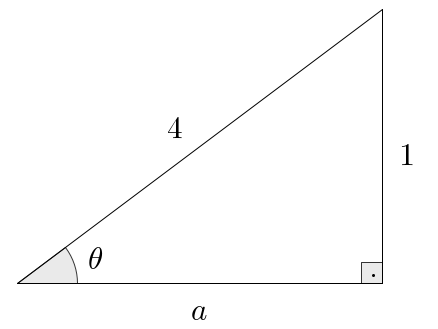
\includegraphics[scale=.3]{./figures/9-1-3-triangle-sin-1-4.png}
        \end{figure}
        So, we find the missing side $a$, using the Pythagorean relation $a^2+b^2=c^2$, which reads and gives: $$a^2+1^2 = 4^2 \implies a^2+1=16\implies a^2=15,$$so that $a=\sqrt{15}$. Now we have all the sides, so finding all the ratios is immediate: $$\sin\theta = \frac{1}{4},\quad \cos\theta=\frac{\sqrt{15}}{4},\quad\mbox{and}\quad\tan\theta=\frac{1}{\sqrt{15}}=\frac{\sqrt{15}}{15}.$$Flipping all the fractions, we obtain$$\csc\theta = 4,\quad \sec\theta=\frac{4\sqrt{15}}{15},\quad\mbox{and}\quad\cot\theta=\sqrt{15}.$$
      \end{itemize}
    \end{explanation}
    
  \item Given: $\cos\theta = 2/3$.

    \begin{explanation}
      \begin{itemize}
      \item {\bf Strategy 1:}       Let's find $\sin\theta$ first, using the first fundamental identity $\sin^2\theta+\cos^2\theta=1$. We have $$\sin^2\theta +\left(\frac{2}{3}\right)^2=1 \implies \sin^2\theta+\frac{4}{9}=1 \implies \sin^2\theta = 1-\frac{4}{9},$$so $$\sin^2\theta = \frac{5}{9} \implies \sin\theta = \frac{\sqrt{5}}{3}.$$ With this, we have that \[   \tan\theta = \frac{\sin\theta}{\cos\theta} = \frac{\sqrt{5}/3}{2/3} = \frac{\sqrt{5}}{2}.  \]Flipping the fractions $$\sin\theta = \frac{\sqrt{5}}{3}, \quad \cos\theta = \frac{2}{3} \quad\mbox{and}\quad \tan\theta = \frac{\sqrt{5}}{2},$$respectively, we obtain $$\csc\theta = \frac{3}{\sqrt{5}}  =\frac{3\sqrt{5}}{5} \quad \sec\theta = \frac{3}{2},\quad\mbox{and}\quad \cot\theta = \frac{2}{\sqrt{5}}=\frac{2\sqrt{5}}{5}.$$
      \item {\bf Strategy 2:} This time, here's the triangle we'll use: \begin{figure}[h]
          \centering
          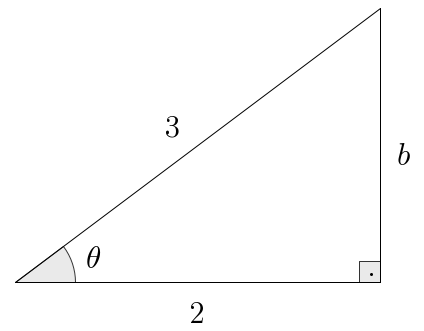
\includegraphics[scale=.3]{./figures/9-1-3-triangle-cos-2-3.png}
        \end{figure} 
        We'll use the Pythagorean relation $a^2+b^2=c^2$ to find the missing side $b$, as follows: $$2^2+b^2=3^2\implies 4+b^2=9\implies b^2=5,$$so $b=\sqrt{5}$. Again, with all the sides, we can read all the main ratios: $$\sin\theta = \frac{\sqrt{5}}{3},\quad\cos\theta=\frac{2}{3},\quad\mbox{and}\quad\tan\theta=\frac{\sqrt{5}}{3}.$$Taking reciprocals, we get the rest:$$\csc\theta = \frac{3\sqrt{5}}{5} \quad \sec\theta = \frac{3}{2},\quad\mbox{and}\quad \cot\theta=\frac{2\sqrt{5}}{5}.$$
      \end{itemize}
    \end{explanation}
    
  \item Given: $\tan\theta = 5/4$.

    \begin{explanation}
      \begin{itemize}
      \item {\bf Strategy 1:} The only fundamental identity we have involving $\tan\theta$ is $\tan^2\theta+1=\sec^2\theta$, so we might as well use it. It reads $$\left(\frac{5}{4}\right)^2 + 1 = \sec^2\theta \implies \sec^2\theta = \frac{25}{16} + 1 \implies \sec^2\theta = \frac{41}{16},$$and so $$\sec\theta = \frac{\sqrt{41}}{4} \implies \cos\theta = \frac{4}{\sqrt{41}} = \frac{4\sqrt{41}}{41}.$$With this, we could in principle find $\sin\theta$, by using $\sin^2\theta+\cos^2\theta=1$ as usual. But there is a simpler way. Namely, we use that $$\tan\theta = \frac{\sin\theta}{\cos\theta} \implies \sin\theta = \tan\theta \cos\theta= \frac{5}{4}\cdot \frac{4\sqrt{41}}{41} \implies \sin\theta = \frac{5\sqrt{41}}{41}.$$Meaning that $$\csc\theta = \frac{\sqrt{41}}{5} \quad\mbox{and}\quad \cot\theta = \frac{4}{5},$$and we are done.
      \item {\bf Strategy 2:} Now, we set a right triangle with legs $4$ and $5$, like below:  \begin{figure}[h]
          \centering
          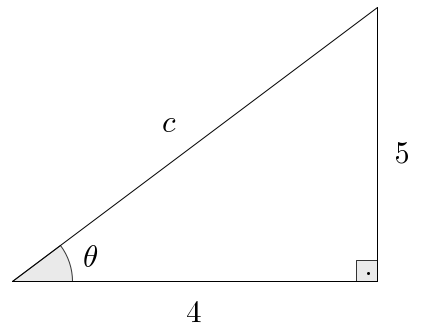
\includegraphics[scale=.3]{./figures/9-1-3-triangle-tan-5-4.png}
        \end{figure} 
      \end{itemize} Since the hypotenuse $c$ is missing, applying the Pythagorean Theorem is even easier: $$c^2 = 4^2+5^2 = 16+25=41\implies c=\sqrt{41}.$$With this in place, we read from the triangle the main ratios as $$\sin\theta=\frac{5\sqrt{41}}{41},\quad \cos\theta=\frac{4\sqrt{41}}{41}\quad\mbox{and}\quad\tan\theta=\frac{5}{4}.$$And taking reciprocals:$$\csc\theta=\frac{\sqrt{41}}{5},\quad \sec\theta=\frac{\sqrt{41}}{4}\quad\mbox{and}\quad\cot\theta=\frac{4}{5}.$$
    \end{explanation}
    
  \item Given: $\sec\theta = 7/3$.

    \begin{explanation}
      \begin{itemize}
      \item {\bf Strategy 1:} We immediately know that $\cos\theta = 3/7$, so let's find $\sin\theta$ next, using the first fundamental identity $\sin^2\theta+\cos^2\theta=1$. We have $$\sin^2\theta +\left(\frac{3}{7}\right)^2=1 \implies \sin^2\theta+\frac{9}{49}=1 \implies \sin^2\theta = 1-\frac{9}{49},$$so $$\sin^2\theta = \frac{40}{49} \implies \sin\theta = \frac{2\sqrt{10}}{7}.$$ With this, we have that \[   \tan\theta = \frac{\sin\theta}{\cos\theta} = \frac{2\sqrt{10}/7}{3/7} = \frac{2\sqrt{10}}{3}.  \]Flipping the remaining fractions $$\sin\theta = \frac{2\sqrt{10}}{7}, \quad\mbox{and}\quad \tan\theta = \frac{2\sqrt{10}}{3},$$respectively, we obtain $$\csc\theta = \frac{7}{2\sqrt{10}}  =\frac{7\sqrt{10}}{20}\quad\mbox{and}\quad \cot\theta = \frac{3}{2\sqrt{10}}=\frac{3\sqrt{10}}{20}.$$
      \item {\bf Strategy 2:} Let's draw a triangle with hypotenuse $7$ and adjacent side to $\theta$ having length $3$: \begin{figure}[h]
          \centering
          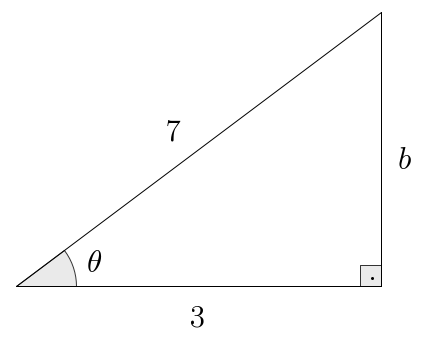
\includegraphics[scale=.3]{./figures/9-1-3-triangle-sec-7-3.png}
        \end{figure}Let's use, as usual, the Pythagorean relation $a^2+b^2=c^2$ to find $b$. It gives us that $$3^2+b^2=7^2\implies 9+b^2=49\implies b^2 = 40\implies b=2\sqrt{10}.$$ 
      \end{itemize}So we have that $$\sin\theta=\frac{2\sqrt{10}}{7},\quad\cos\theta=\frac{3}{7},\quad\mbox{and}\quad \tan\theta=\frac{2\sqrt{10}}{3}.$$Taking reciprocals and rationalizing each of them, we also get$$\csc\theta=\frac{7\sqrt{10}}{20},\quad\sec\theta=\frac{7}{3},\quad\mbox{and}\quad \cot\theta=\frac{3\sqrt{10}}{20}.$$
    \end{explanation}
    
  \item Given: $\csc\theta = 8/7$.

    \begin{explanation}
      \begin{itemize}
      \item {\bf Strategy 1:} We immediately know that $\sin\theta = 7/8$, so let's find $\cos\theta$ next, using the first fundamental identity $\sin^2\theta+\cos^2\theta=1$. We have $$\left(\frac{7}{8}\right)^2+\cos^2\theta=1 \implies \frac{49}{64}+\cos^2\theta=1 \implies \cos^2\theta = 1-\frac{49}{64},$$so $$\cos^2\theta = \frac{15}{64} \implies \cos\theta = \frac{\sqrt{15}}{8}.$$ With this, we have that \[   \tan\theta = \frac{\sin\theta}{\cos\theta} = \frac{7/8}{\sqrt{15}/8} = \frac{7}{\sqrt{15}} = \frac{7\sqrt{15}}{15}.  \]Flipping the remaining fractions $$\cos\theta = \frac{\sqrt{15}}{8}, \quad\mbox{and}\quad \tan\theta = \frac{7}{\sqrt{15}},$$respectively, we obtain $$\sec\theta = \frac{8}{\sqrt{15}} =\frac{8\sqrt{15}}{15} \quad\mbox{and}\quad \cot\theta =\frac{\sqrt{15}}{7}.$$
      \item {\bf Strategy 2:} Consider the following triangle: \begin{figure}[h]
          \centering
          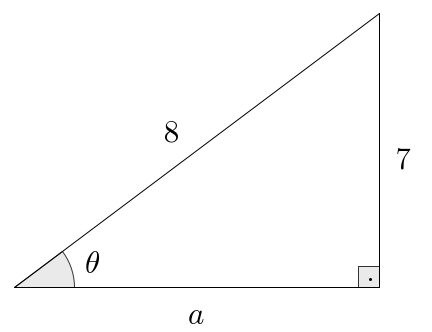
\includegraphics[scale=.3]{./figures/9-1-3-triangle-csc-8-7.png}
        \end{figure}Let's find $a$ using the Pythagorean relation $a^2+b^2=c^2$, which becomes $$a^2+7^2=8^2\implies a^2+49=64\implies a^2 = 15,$$so that $a=\sqrt{15}$. Having all the sides of the triangle, we read that $$\sin\theta=\frac{7}{8},\quad\cos\theta=\frac{\sqrt{15}}{8},\quad\mbox{and}\quad\tan\theta=\frac{7\sqrt{15}}{15}.$$Taking reciprocals, we get $$\csc\theta=\frac{8}{7},\quad\sec\theta=\frac{8\sqrt{15}}{15},\quad\mbox{and}\quad\cot\theta=\frac{\sqrt{15}}{7}$$ as well.
      \end{itemize}
    \end{explanation}
    
  \item Given: $\cot\theta = 2/9$.

    \begin{explanation}
      \begin{itemize}
      \item {\bf Strategy 1:} We immediately know that $\tan \theta = 9/2$ and, again, the only fundamental identity we have involving $\tan\theta$ is $\tan^2\theta+1=\sec^2\theta$. It reads $$\left(\frac{9}{2}\right)^2 + 1 = \sec^2\theta \implies \sec^2\theta = \frac{81}{4} + 1 \implies \sec^2\theta = \frac{85}{4},$$and so $$\sec\theta = \frac{\sqrt{85}}{2} \implies \cos\theta = \frac{2}{\sqrt{85}} = \frac{2\sqrt{85}}{85}.$$Again, instead of using $\sin^2\theta+\cos^2\theta=1$ to find $\sin\theta$, we can just argue that $$\tan\theta = \frac{\sin\theta}{\cos\theta} \implies \sin\theta = \tan\theta \cos\theta= \frac{9}{2}\cdot \frac{2\sqrt{85}}{85} \implies \sin\theta = \frac{9\sqrt{85}}{85}.$$Meaning that $$\csc\theta = \frac{\sqrt{85}}{9},$$and so we are done.

        As an aside, try to solve this problem again without immediately using that $\tan\theta=9/2$, start only with $\cot\theta =2/9$, use the identity $1+\cot^2\theta=\csc^2\theta$ and go from there, it is instructive.
      \item {\bf Strategy 2:} Again, let's set up a convenient triangle: \begin{figure}[h]
          \centering
          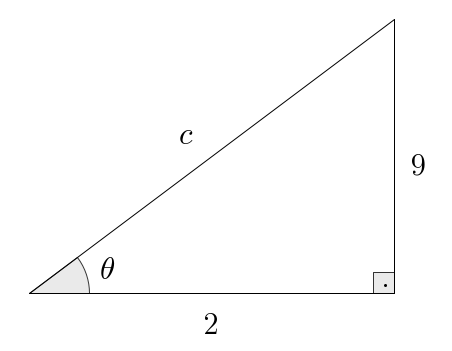
\includegraphics[scale=.3]{./figures/9-1-3-triangle-cot-2-9.png}
        \end{figure} Here, in particular, note that the scale and proportions in this picture are completely off. This is ok, since drawing triangles is just meant to help us organize what is the opposite side to $\theta$, what is the adjacent side, and what is the hypotenuse. It doesn't matter how bad your picture looks, as long as the ``positions'' are correct. In any case, we immediately find $c$ with $$c^2=a^2+b^2=2^2+9^2 = 4+81=85,$$so $c=\sqrt{85}$. Now we can read all the ratios and rationalize them to obtain: $$\sin\theta=\frac{9\sqrt{85}}{85},\quad\cos\theta=\frac{2\sqrt{85}}{85},\quad\mbox{and}\quad\tan\theta=\frac{9}{2}.$$Take reciprocals and rationalize whatever is needed to get $$\csc\theta=\frac{\sqrt{85}}{9},\quad\sec\theta=\frac{\sqrt{85}}{2},\quad\mbox{and}\quad\cot\theta=\frac{2}{9}$$as well.
      \end{itemize}
    \end{explanation}
  \end{enumerate}
\end{example}

Let's summarize the highlights of the strategy, from the algebraic perspective.

\begin{enumerate}
\item If you're given $\sin$ or $\cos$, use the fundamental identity to find the other one. Then find $\tan=\sin/\cos$, and flip all the fractions to get $\csc$, $\sec$ and $\tan$.
\item If you're given $\csc$ or $\sec$, flip it to get $\sin$ or $\cos$, and proceed as (a).
\item If you're given $\tan$, use $\tan^2\theta+1=\sec^2\theta$ to find $\sec\theta$. Once you have $\sec\theta$, you have $\cos\theta$. Then proceed as (a).
\item If you're given $\cot$, flip it to get $\tan$, and proceed as (c).
\end{enumerate}

Note that we're employing a mathematician's general philosophy here: take a problem and reduce it to something which you already know how to solve (namely, we're arguing that --- morally --- if you know how to solve the problem when you were given either $\sin$ or $\cos$, then you in fact know how to solve it when given \emph{any} of the six trigonometric functions). And also from the geometric perspective, the strategy is even easier to describe: recognize the trigonometric function you were given in terms of ${\rm opp.}$, ${\rm adj.}$ and ${\rm hyp.}$, then draw a right triangle with this information. You will be missing one side, which can be found with the Pythagorean Theorem. Once you have all sides, you can find all the ratios between sides.

Of course, the two above ways to go about this are not the only ones, but they're as good a recipe as any. In any case, you have room for creativity here. And even if one method seems easier than the other, it is useful to be comfortable with both, as this is already a good chance to start getting acquainted with trigonometry identities, which will be indispensable later.

We will see later how to define and deal with trigonometric functions for angles which are not necessarily acute. Then, everything we did here becomes slightly more subtle, as one must now pay attention to signs (for example, we'll have that $\cos(120^\circ) = -1/2$). But the overall program of using the fundamental trigonometric identities and the relations between the main trigonometric functions ($\sin$, $\cos$, and $\tan$) with their reciprocals ($\csc$, $\sec$, and $\cot$) will always be useful.


%\typeout{************************************************}
%\typeout{Summary}
%\typeout{************************************************}

\begin{summary}\begin{itemize}
\item We have illustrated, with several examples, two ways to find all the values of the trigonometric functions at an acute angle $\theta$, once we know one of the values. This can be done algebraically by exploring trigonometric identities, or geometrically by drawing the ``correct'' triangle and applying the Pythagorean Theorem to find the missing side -- to then read all ratios directly from the triangle itself.
\end{itemize}\end{summary}




\end{document}
